This chapter provides an overview of the basic concepts needed to understand the problem of optimizing electric vehicle charging station infrastructure. It discusses electric vehicles and their charging needs, multi-objective optimization (MOO), evolutionary algorithms (EAs), and multi-objective evolutionary algorithms (MOEAs), and specifically the NSGA-II algorithm, which is a central method in this study.

\section{Electric Vehicles and Charging Infrastructure}

The use of electric vehicles has increased in recent years, driven by growing concerns about climate change. Government policies promoting sustainable transportation have significantly fueled this growth.

In addition, advances in battery technology have played a key role in supporting this shift, as they have become more affordable and accessible. All of these factors have significantly contributed to accelerating the adoption of electric vehicles.

Moreover, gasoline and diesel vehicles can be developed to handle large amounts of fuel at a reasonable cost and can be refueled quickly and easily. However, despite significant advances in battery technology, electric vehicles face the challenge of increasing their battery capacity due to their high cost, making a reliable and accessible charging network important.



There are generally three levels of EV chargers:
\begin{itemize}
    \item \textbf{AC Level 1 Charging:} Level 1 charging is the most basic method to charge an electric vehicle (EV). It uses a standard 120-volt household outlet. This charger level is often used when no other higher voltage charging options are available. Although this type of charger is very slow, it is still practical for many drivers, especially those who drive short distances every day. Level 1 charging is simple and requires no installation. Most electric cars come with a Level 1 charging cable that can be plugged directly into a household electrical outlet.
    Moreover, Level 1 charging meets simple daily needs. For example, charging an electric car for 8 hours increases its driving range to approximately 64 kilometers (40 miles). This is sufficient for normal daily driving. Overall, Level 1 charging may not be ideal for long-distance travel, but for many EV owners, it offers a cost effective and easy way to charge at home without needing extra equipment\cite{Alternative Fuels Data Center}.

        
    \item \textbf{AC Level 2 Charging:} Level 2 charging provides electric vehicle (EV) charging through a 240 volt electrical supply in residential settings, or 208 volts in commercial environments\cite{Alternative Fuels Data Center}. Unlike Level 1 charging, which uses a standard 120V outlet and charges slowly, Level 2 significantly reduces charging time, making it a popular choice for both home and public use. Level 2 charging is much faster than Level 1, using a 220V outlet instead of the standard 120V\cite{Alternative Fuels Data Center}. This significantly reduces charging time, making it a popular choice for both home and public use. One of the main benefits of Level 2 charging is its ability to fully charge a typical EV battery overnight. This makes it ideal for daily use.

    However, Level 2 equipment is also widely used at public stations, workplaces, and shopping centers to support EV users. Overall, Level 2 charging offers a good balance between speed and efficiency, making it the preferred choice for many EV users.
    
    \item \textbf{DC Fast Charging:} Level 3 charging operates at around 400 volts, allowing electric vehicles (EVs) to charge significantly faster than with standard Level 1 or Level 2 charging\cite{DC Fast Chargers for Electric Vehicles}.   
    
    
    This technology provide up to 500 kilowatts (kW) of power, making it ideal for busy highways and transportation routes where fast charging is crucial\cite{Alternative Fuels Data Center}.
    In addition, DC fast charging stations are especially useful for long-distance travel and commercial applications, as they can recharge an EV battery to 80\% in as little as 20–30 minutes, depending on the vehicle and charger capacity\cite{Alternative Fuels Data Center}.

    The growing adoption of medium and heavy duty electric vehicles (EVs) such as electric buses, delivery vans, and heavy trucks increased demand for DC fast charging infrastructure. These vehicles have larger batteries, which requiring higher charging capacities. 
    
    Overall, DC fast charging plays a critical role in supporting the widespread adoption of EVs across personal, commercial, and public transportation sectors.
\end{itemize}

Figure 2.1 shows the distribution of charger levels in use in the United States\cite{Alternative Fuels Data Center}.

\begin{figure}[h!]
\centering
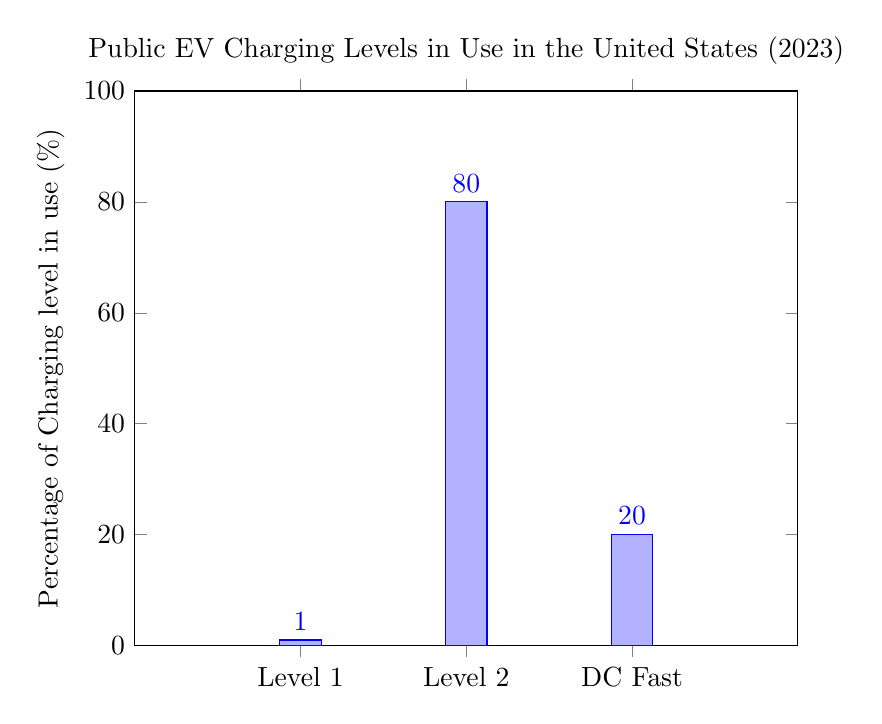
\begin{tikzpicture}
\begin{axis}[
    ybar,
    symbolic x coords={Level 1, Level 2, DC Fast},
    xtick=data,
    ylabel={Percentage of Charging level in use (\%)},
    ymin=0, ymax=100,
    width=10cm,
    bar width=15pt,
    nodes near coords,
    enlarge x limits=0.5,
    title={Public EV Charging Levels in Use in the United States (2023)}
]
\addplot coordinates {(Level 1, 1) (Level 2, 80) (DC Fast, 20)};
\end{axis}
\end{tikzpicture}
\caption{Distribution of EV Charging Port Types in the United States (2023)}
\end{figure}

Connectors for electric vehicle (EV) charging vary depending on the region and charging level. Generally, the standard SAE J1772 connector is widely used for both Level 1 and Level 2 charging. For Level 3, or DC fast charging, the most commonly used connectors are the Combined Charging System (CCS) and CHAdeMO\cite{Alternative Fuels Data Center}.

Moreover, Tesla, as a major player in the EV industry, uses a proprietary connector for its vehicles. However, it also provides compatibility with the CCS connector through the use of adapters\cite{Alternative Fuels Data Center}.

Figure 2.2 illustrates the types of connectors used for Levels 1, 2, and 3.


\begin{figure}[h]
    \centering
    \includegraphics[width=0.8\textwidth]{../Figures/EV_connecters.PNG}
    \caption{Types of EV connectors used for Levels 1, 2, and 3 \cite{Alternative Fuels Data Center}}
    \label{fig:EV connectors}
\end{figure}

\clearpage
Figure 2.3 illustrates the relationship between average charging speed and charging time for the three levels of electric vehicle (EV) charging based on data from the U.S. Department of Transportation \cite{U.S. Department of Transportation}. Level 1 charging has the longest average charging time of approximately 65 hours, and delivers the lowest charging speed of around 5 miles per hour. In contrast, Level 2 charging reduces the charging time to an average of 5.5 hours and increases the average charging speed to 46 miles per hour. Level 3 charging, or DC fast charging, offers the highest efficiency with an average charging time of just 0.75 hours and a substantial charging speed of approximately 638 miles per hour. 

\begin{figure}[h]
    \centering
    \includegraphics[width=0.8\textwidth]{../Figures/EVC_Levels.png}
    \caption{Average charging speed versus charging time for different EV charging levels}
    \label{fig:EVC Levels}
\end{figure}


This clear trend highlights the performance differences between charging levels, with faster charging options offering significantly higher power output and reduced wait times. These differences are crucial for consumers and EV charging station operators when choosing the right charging infrastructure to meet their specific operational needs. This clearly contributes to supporting the spread and convenience of EV.




\section{Multi-Objective Optimization (MOO)}
Multi Objective Optimization (MOO) seeks to optimize multiple conflicting objectives simultaneously. Unlike single-objective optimization, which produces one best solution, MOO generates a set of Pareto optimal solutions\cite{Multi-Objective Optimization using Evolutionary Algorithms}. 

In addition, these solutions represent trade-offs, where improving one objective results in worsening another. The set of all Pareto optimal solutions forms the Pareto front, which shows the best possible trade-offs between the objectives. Each point on this front represents a solution where no objective can be improved without degrading another. MOO is commonly used in complex decision-making problems where multiple criteria must be considered. It provides valuable insights into the balance between competing objectives.\cite{Multi-Objective Optimization using Evolutionary Algorithms}.

Regarding \cite{Nonlinear multiobjective optimization} The general expression of a multi objective optimization (MOO) problem:
\[
\text{Minimize } \mathbf{F}(x) = [f_1(x), f_2(x), \ldots, f_k(x)], \quad \text{subject to } x \in \Omega
\]

where 
\begin{itemize}
  \item \textbf{\( \mathbf{F}(x) \)}: Represents the vector of \( k \) objective functions. Each \( f_i(x) \) corresponds to a distinct goal or objective, and the decision vector \( x \) influences all of them.
  
  \item \textbf{\( \Omega \)}: Refers to the feasible set of decision variables, which defines the constraints the decision variables must satisfy.
  
  \item \textbf{Minimization}: The aim is typically to minimize each objective function, although maximization is also common. In many cases, improving one objective could negatively affect another, creating trade-offs that are a key challenge in multi-objective optimization.
\end{itemize}


MOO is used across many domains:

- \textbf{Engineering}: Balancing trade-offs among cost, weight, and performance.
- \textbf{Energy Systems}: Optimizing efficiency, cost, and environmental impact \cite{Multi-objective}.
- \textbf{Finance}: Portfolio optimization involving return and risk.
- \textbf{Machine Learning}: Hyperparameter tuning involving accuracy, complexity, and fairness \cite{An efficient neural architecture search system}.


\subsection{Trade-offs in Multi-Objective Optimization: The Role of Pareto Optimality}

In multi-objective optimization (MOO), it is often impossible to identify a single solution that optimally satisfies all objectives simultaneously, especially when the objectives conflict \cite{Nonlinear multiobjective optimization}. Instead, the goal is to find a set of solutions that represent acceptable trade-offs. A solution is considered \textit{Pareto optimal} if there is no other feasible solution that can improve at least one objective without worsening another. According the principle of MOO, Pareto optimality plays a crucial role in evaluating the quality of a solution amidst conflicting objectives \cite{Nonlinear multiobjective optimization}.

The collection of all Pareto optimal solutions is known as the \textit{Pareto front}. Each point on this front represents a non-dominated solution, meaning that no other solution in the feasible space is strictly better in all objectives. As such, the Pareto front provides decision-makers with a spectrum of choices, each embodying different trade-offs among the objectives. This allows for flexibility in selecting solutions that align with specific priorities or operational constraints \cite{Nonlinear multiobjective optimization}.

In addition, identifying the Pareto front supports more informed decision-making, particularly in complex systems where multiple performance metrics must be balanced. For example, in engineering design, a solution may involve trade-offs between cost, efficiency, and robustness. In such scenarios, a decision-maker might prioritize cost-effectiveness while ensuring that other performance criteria remain within acceptable limits \cite{Nonlinear multiobjective optimization}.

However, selecting a single solution from the Pareto front is not trivial. This process typically involves incorporating decision-maker preferences, which may be explicit (e.g., assigning weights to objectives) or implicit (e.g., using interactive methods). Furthermore, these preferences may change over time or remain uncertain, adding another layer of complexity to the optimization process \cite{Survey of multi-objective optimization methods}.

Understanding trade-offs among objectives and visualizing the Pareto front play a vital role in revealing interactions between decision variables, defining the limits of achievable performance, and supporting strategic decision-making \cite{Nonlinear multiobjective optimization}. 

The shape of the Pareto front can impact the performance of optimization methods. Classical methods, like the weighted sum approach. In contrast, evolutionary algorithms are better at exploring different areas of the Pareto front because they use a population-based method and can handle complex, nonlinear problems \cite{Nonlinear multiobjective optimization}.

In summary, Pareto optimality provides a rigorous framework for analyzing and interpreting trade-offs in multi-objective problems. It serves as a decision support mechanism, helping stakeholders to navigate complex trade-offs and make choices that best align with their objectives and constraints.

\subsection{Solution Methods}
Several methods have been developed to solve Multi-Objective Optimization (MOO) problems, categorized into classical and evolutionary approaches. Both approaches provide valuable tools depending on the nature of the problem. Classical methods tend to be more straightforward, but may face limitations with complex, high-dimensional problems. Evolutionary algorithms, on the other hand, are well suited for handling such complexity and are the primary focus of this research.

\textbf{Classical Methods}: In classical Multi-Objective Optimization (MOO), scalarization techniques are commonly employed to simplify the problem by converting multiple objectives into a single objective function. One such technique is the weighted sum method, where each objective is assigned a weight and then combined into a single function. This method is computationally efficient and performs well when the Pareto front is smooth and regular. However, it may fail in cases where the Pareto front is non-smooth or discontinuous, as it might not capture all potential solutions. Another widely used classical method is the \(\epsilon\) constraint method. In this approach, one objective is optimized, while the other objectives are constrained within specific bounds. Although this method ensures that all objectives are considered, it requires multiple runs with different constraint settings to fully explore the Pareto front. While classical methods are efficient for low-dimensional problems, they tend to struggle with high-dimensional, nonlinear, or complex objective landscapes \cite{Nonlinear multiobjective optimization}, \cite{Multi-Objective Optimization using Evolutionary Algorithms}.


\textbf{Evolutionary Algorithms (EAs)}: 

Evolutionary Algorithms (EAs) are population-based, stochastic optimization techniques inspired by the principles of natural selection and genetics \citep{Evolutionary algorithms in theory and practice},\cite{Multi-Objective Optimization using Evolutionary Algorithms}. They employ biologically inspired operations such as selection, crossover, and mutation to iteratively evolve a set of candidate solutions toward optimal or near-optimal trade-offs across multiple objectives.

The general structure of an EA consists of the following steps \cite{Multi-Objective Optimization using Evolutionary Algorithms}:
\begin{enumerate}
    \item \textbf{Initialization:} Generate an initial population of solutions randomly or heuristically.
    \item \textbf{Evaluation:} Assess the fitness of each individual using the defined objective functions.
    \item \textbf{Selection:} Choose high quality solutions based on fitness to serve as parents for the next generation.
    \item \textbf{Variation:} Apply genetic operators such as crossover and mutation to generate new offspring.
    \item \textbf{Replacement:} Form a new generation by selecting individuals from the current population and the offspring.
\end{enumerate}

EAs are particularly effective for tackling complex, nonlinear, and high dimensional optimization problems where classical methods may struggle, especially when the Pareto front is irregular \cite{Evolutionary algorithms in theory and practice}. Its strength lies in its ability to maintain a diverse set of solutions, which allows it to explore different regions of the solution space simultaneously. This makes it particularly suitable for multi objective optimization problems.



\textit{Given these advantages, this research focuses on applying evolutionary algorithms as a fundamental framework for optimization, leveraging their flexibility and robustness in dealing with complex trade-offs in multi-objective problems.}

\section{Multi-Objective Evolutionary Algorithms (MOEAs)}

Multi-objective evolutionary algorithms (MOEAs) are extensions of traditional evolutionary algorithms designed to address problems with multiple, often conflicting, objectives. Unlike single-objective evolutionary algorithms, MOEAs maintain a set of solutions, allowing multiple solutions to be explored simultaneously \citep{Evolutionary Multi-objective Optimization: A Historical View of the Field}.

According to \citep{Evolutionary Multi-objective Optimization: A Historical View of the Field}, the key features of MOEAs are as follows:

\begin{itemize}
    \item \textbf{Diversity Preservation:} Mechanisms such as crowding distance and niching ensure a well-distributed set of solutions across the Pareto front.
    \item \textbf{Pareto Dominance:} Selection is based on dominance relations, where one solution dominates another if it is no worse in all objectives and better in at least one.
    \item \textbf{Archiving:} High-quality non-dominated solutions are stored in an external archive to preserve progress across generations.
\end{itemize}

MOEA models have been widely applied in various fields, including engineering design, logistics, supply chain optimization, telecommunications, and power systems planning, due to their ability to handle complex, nonlinear, and high-dimensional objective spaces \cite{Evolutionary Multi-objective Optimization: A Historical View of the Field}.

\section{NSGA-II Algorithm}

The Non-dominated Sorting Genetic Algorithm II (NSGA-II), proposed by Deb et al. \cite{IEEE Transactions on Evolutionary Computation}, is one of the most popular and efficient Multi-Objective Evolutionary Algorithms (MOEAs).

According \cite{IEEE Transactions on Evolutionary Computation} , NSGA-II introduces several key innovations as follows:
\begin{itemize}
    \item \textbf{Fast Non-dominated Sorting:} This method efficiently classifies the population into different levels of non-domination, ensuring the diversity of solutions.
    \item \textbf{Crowding Distance:} Measures the density of solutions surrounding a particular solution, promoting diversity by maintaining a spread of solutions across the objective space.
    \item \textbf{Elitism:} Retains the best solutions of individuals across generations, ensuring that the quality of the population improves over time.
\end{itemize}

The algorithm can be summarized in the following steps \cite{IEEE Transactions on Evolutionary Computation}:

\begin{enumerate} \item Combine the parent and offspring populations into one single population. \item Rank the combined population by non-dominance, categorizing solutions into different levels. \item Select the best individuals based on crowding distance, ensuring diversity is preserved, until the next generation is complete. \item Apply variation operators (crossover and mutation) to generate offspring for the subsequent generation. \end{enumerate}


In addition, NSGA-II is computationally efficient, with a time complexity of \(O(MN^2)\), where \(M\) is the number of objectives and \(N\) is the population size \cite{IEEE Transactions on Evolutionary Computation}. Its ability to balance convergence and diversity makes it highly suitable for solving complex multi objective problems, such as Electric Vehicle Charging Station (EVCS) optimization. This matches well with the objectives of this research, which are to maximize coverage, maximize charger speed to reduce waiting times, minimize the number of stations, minimize the number of chargers, and minimize the average distance to stations. NSGA-II explores a variety of possible charging solutions and converges toward Pareto-optimal solutions, effectively addressing the trade-offs between these conflicting objectives. By efficiently handling these goals, NSGA-II proves to be a powerful tool for optimizing the design of EVCS, Ensuring efficiency and coverage while reducing wait times and lowering overall costs.


